\documentclass[11pt,a4paper]{article}
\usepackage[margin=2.3cm]{geometry}
\usepackage{amsmath,amssymb}
\usepackage{graphicx}
\usepackage{booktabs}
\usepackage{hyperref}
\usepackage{tikz}
\usepackage{float}
\usetikzlibrary{positioning}

\title{Reproduccion alternativa de gradient pathologies en PINNs\\
\large Difusion de calor 1D en una barra metalica}
\author{Trabajo practico de Optimizacion}
\date{Mayo 2026}

\begin{document}
\maketitle

\begin{abstract}
Se replica el nucleo metodologico de Wang, Teng y Perdikaris
(\emph{Understanding and mitigating gradient pathologies in physics-informed
neural networks}) sobre un problema distinto: difusion de calor unidimensional
en una barra metalica. Se comparan una PINN clasica (M1), una PINN con balance
adaptativo de terminos de perdida basado en estadisticas de gradientes (M2) y
la solucion analitica del problema. No se implementa la arquitectura nueva del
paper. Tambien se incluye busqueda bayesiana de hiperparametros y una
comparacion de optimizadores.
\end{abstract}

\section{Problema fisico}

La barra tiene longitud $L=1\,\mathrm{m}$, difusividad termica
$\alpha=10^{-4}\,\mathrm{m^2/s}$, extremos mantenidos a temperatura ambiente
$T_{\mathrm{amb}}=20^\circ\mathrm{C}$ y escala de temperatura
$\Delta T=80^\circ\mathrm{C}$. La ecuacion dimensional es
\begin{equation}
  \frac{\partial T}{\partial t}
  = \alpha \frac{\partial^2 T}{\partial X^2},
  \qquad 0<X<L,\quad t>0.
\end{equation}
Las condiciones de borde son
\begin{equation}
  T(0,t)=T(L,t)=T_{\mathrm{amb}}.
\end{equation}

\begin{figure}[H]
\centering
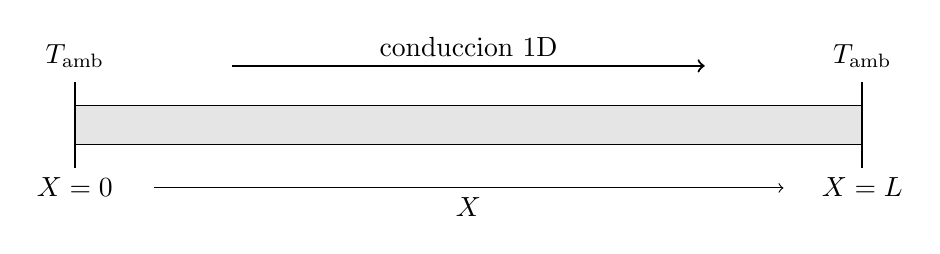
\begin{tikzpicture}[scale=1.0]
  \draw[very thick] (0,0) -- (10,0);
  \draw[fill=gray!20] (0,-0.25) rectangle (10,0.25);
  \draw[thick] (0,-0.55) -- (0,0.55);
  \draw[thick] (10,-0.55) -- (10,0.55);
  \node[below] at (0,-0.55) {$X=0$};
  \node[below] at (10,-0.55) {$X=L$};
  \node[above] at (0,0.6) {$T_{\mathrm{amb}}$};
  \node[above] at (10,0.6) {$T_{\mathrm{amb}}$};
  \draw[->,thick] (2,0.75) -- (8,0.75);
  \node[above] at (5,0.75) {conduccion 1D};
  \draw[->] (1,-0.8) -- (9,-0.8);
  \node[below] at (5,-0.8) {$X$};
\end{tikzpicture}
\caption{Sistema de referencia para la barra metalica.}
\end{figure}

Se adimensionaliza con
\begin{equation}
  x=\frac{X}{L},\qquad
  \tau=\frac{\alpha t}{L^2},\qquad
  u=\frac{T-T_{\mathrm{amb}}}{\Delta T}.
\end{equation}
El problema usado por la PINN es entonces
\begin{align}
  u_\tau-u_{xx} &= 0,
  &&0<x<1,\quad 0<\tau<\tau_f,\\
  u(0,\tau)&=u(1,\tau)=0,\\
  u(x,0)&=u_0(x),
\end{align}
donde $\tau_f=0.25$, equivalente a $t_f=2500\,\mathrm{s}$.

La condicion inicial es una suma de modos compatibles con los bordes:
\begin{equation}
  u_0(x)=\sin(\pi x)+0.5\sin(3\pi x)+0.25\sin(5\pi x).
\end{equation}
La solucion analitica por separacion de variables es
\begin{equation}
  u(x,\tau)=\sum_{n\in\{1,3,5\}} a_n
  \sin(n\pi x)\exp\left(-(n\pi)^2\tau\right),
\end{equation}
con $(a_1,a_3,a_5)=(1,0.5,0.25)$.

\section{Datos generados para la PINN}

No se usa un dataset fijo de interior. En cada iteracion se generan nuevos
minibatches:
\begin{align}
  x_r &\sim \mathcal{U}(0,1),&
  \tau_r &\sim \mathcal{U}(0,\tau_f) && \text{residuo},\\
  x_0 &\sim \mathcal{U}(0,1),&
  \tau_0 &= 0 && \text{condicion inicial},\\
  \tau_b &\sim \mathcal{U}(0,\tau_f),&
  x_b &\in \{0,1\} && \text{bordes}.
\end{align}
En la corrida final se usa batch $256$ para residuo, condicion inicial y borde.
La mitad del batch de borde esta en $x=0$ y la otra mitad en $x=1$.

La grilla de evaluacion es regular, con $n_x=n_\tau=180$. El error reportado es
\begin{equation}
  \varepsilon_{L^2}=
  \frac{\lVert u_\theta-u_{\mathrm{exacta}}\rVert_2}
       {\lVert u_{\mathrm{exacta}}\rVert_2}.
\end{equation}

\section{PINN y perdidas}

La red $u_\theta(x,\tau)$ es una MLP totalmente conectada con activacion
$\tanh$. Antes del primer layer se escala la entrada a $[-1,1]^2$:
\begin{equation}
  z = 2\frac{[x,\tau]-[0,0]}{[1,\tau_f]-[0,0]}-1.
\end{equation}
La inicializacion es Xavier normal para pesos y cero para sesgos. La arquitectura
principal final es
\begin{equation}
  [2,50,50,50,1].
\end{equation}

Las perdidas son
\begin{align}
  L_{\mathrm{res}} &= \mathrm{mean}\left((u_\tau-u_{xx})^2\right),\\
  L_{\mathrm{ic}}  &= \mathrm{mean}\left((u_\theta(x,0)-u_0(x))^2\right),\\
  L_{\mathrm{bc}}  &= \mathrm{mean}\left(u_\theta(0,\tau)^2+
                     u_\theta(1,\tau)^2\right).
\end{align}
Las derivadas $u_\tau$ y $u_{xx}$ se calculan con autograd de PyTorch.

\section{Modelos comparados}

El baseline M1 minimiza
\begin{equation}
  L_{\mathrm{M1}}=L_{\mathrm{res}}+L_{\mathrm{ic}}+L_{\mathrm{bc}}.
\end{equation}

El modelo M2 usa la correccion de balance adaptativo del paper:
\begin{equation}
  L_{\mathrm{M2}}=
  L_{\mathrm{res}}+\lambda_{\mathrm{ic}}L_{\mathrm{ic}}
  +\lambda_{\mathrm{bc}}L_{\mathrm{bc}}.
\end{equation}
Cada 10 iteraciones se estiman pesos instantaneos
\begin{equation}
  \widehat{\lambda}_i =
  \frac{\max_\theta |\nabla_\theta L_{\mathrm{res}}|}
       {\mathrm{mean}_\theta |\nabla_\theta L_i|},
  \qquad i\in\{\mathrm{ic},\mathrm{bc}\},
\end{equation}
y se actualizan con media movil
\begin{equation}
  \lambda_i \leftarrow
  \beta\lambda_i+(1-\beta)\widehat{\lambda}_i.
\end{equation}
En la corrida final se usa $\beta=0.9$. Las estadisticas se computan sobre los
pesos de las capas lineales, como en el repositorio de los autores.

\begin{figure}[H]
\centering
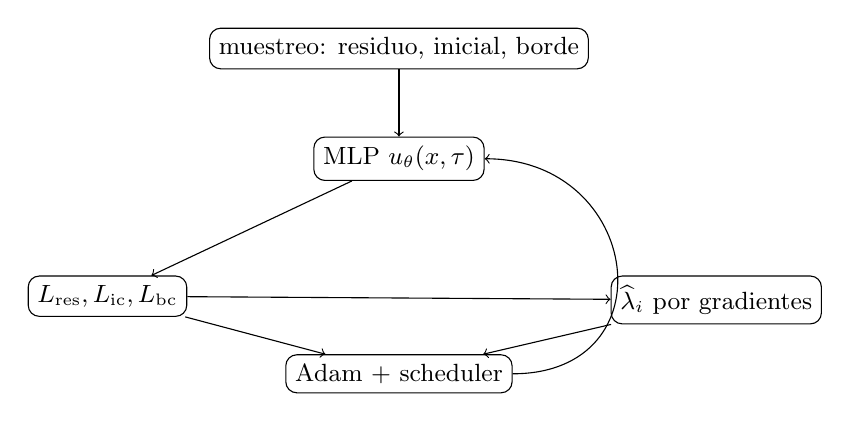
\begin{tikzpicture}[node distance=1.4cm, every node/.style={font=\small}]
  \node[draw, rounded corners] (sample) {muestreo: residuo, inicial, borde};
  \node[draw, rounded corners, below of=sample] (net) {MLP $u_\theta(x,\tau)$};
  \node[draw, rounded corners, below left=1.2cm and 1.6cm of net] (losses) {$L_{\mathrm{res}},L_{\mathrm{ic}},L_{\mathrm{bc}}$};
  \node[draw, rounded corners, below right=1.2cm and 1.6cm of net] (lambdas) {$\widehat{\lambda}_i$ por gradientes};
  \node[draw, rounded corners, below=2.2cm of net] (step) {Adam + scheduler};
  \draw[->] (sample) -- (net);
  \draw[->] (net) -- (losses);
  \draw[->] (losses) -- (lambdas);
  \draw[->] (losses) -- (step);
  \draw[->] (lambdas) -- (step);
  \draw[->] (step.east) .. controls +(2,0) and +(2,0) .. (net.east);
\end{tikzpicture}
\caption{Flujo de entrenamiento para M2. M1 usa el mismo flujo sin actualizar
pesos adaptativos.}
\end{figure}

\section{Optimizacion e hiperparametros}

La corrida principal usa Adam con learning rate inicial $10^{-3}$, sin
weight decay, semilla 0, CPU y 16 threads. El scheduler es exponencial:
\begin{equation}
  \eta_k=\eta_0\left(0.9^{1/1000}\right)^k.
\end{equation}
El entrenamiento principal dura 3000 iteraciones.

La busqueda bayesiana usa Optuna/TPE con 8 trials y 800 iteraciones por trial.
El espacio explorado fue:
\begin{center}
\begin{tabular}{ll}
\toprule
Parametro & Rango \\
\midrule
ancho & $\{24,32,48,64,80\}$ \\
profundidad & enteros de 2 a 5 \\
learning rate & log-uniforme en $[10^{-4},3\cdot 10^{-3}]$ \\
batch & $\{128,256,384\}$ \\
$\beta$ adaptativo & uniforme en $[0.75,0.97]$ \\
\bottomrule
\end{tabular}
\end{center}

\section{Resultados}

\begin{table}[H]
\centering
\begin{tabular}{lrrrr}
\toprule
Modelo & error $L^2$ rel. & tiempo [s] & $\lambda_{\mathrm{ic}}$ & $\lambda_{\mathrm{bc}}$ \\
\midrule
M1 & 0.293134 & 134.47 & 1.00 & 1.00 \\
M2 & 0.102912 & 421.23 & 219148.36 & 276036.68 \\
\bottomrule
\end{tabular}
\caption{Comparacion principal con arquitectura $[2,50,50,50,1]$ y 3000 iteraciones.}
\end{table}

La mejora de M1 a M2 fue $2.85\times$ en error relativo $L^2$.

\begin{figure}[H]
\centering
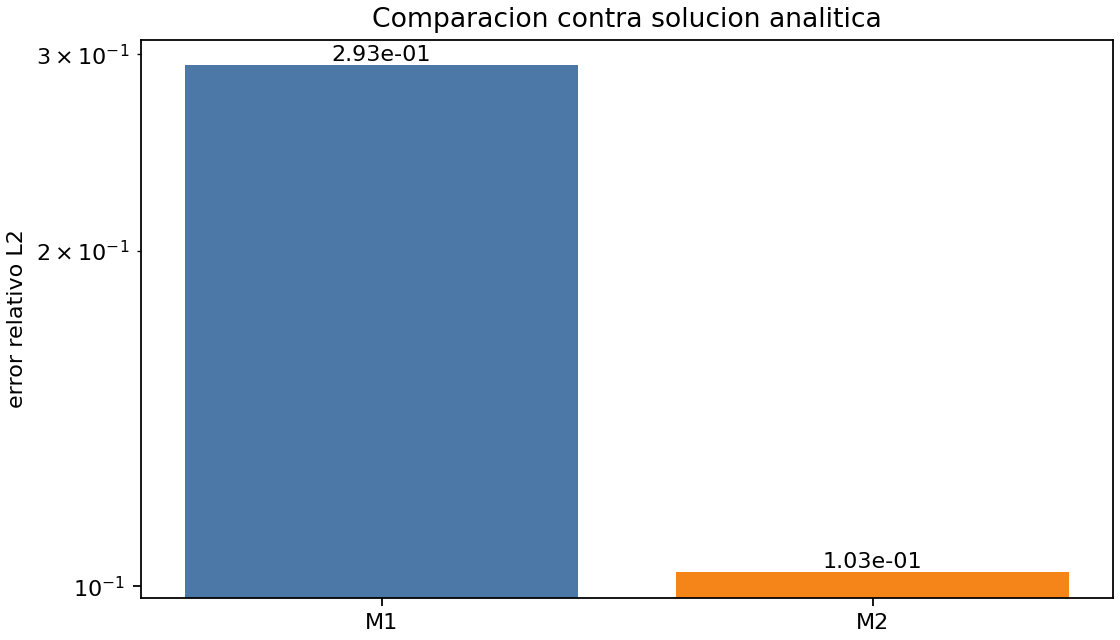
\includegraphics[width=0.70\linewidth]{outputs/comparacion_modelos.png}
\caption{Error relativo $L^2$ contra solucion analitica.}
\end{figure}

\begin{figure}[H]
\centering

\includegraphics[width=\linewidth]{outputs/M1_solucion.png}
\caption{Solucion exacta, prediccion M1 y error absoluto.}
\end{figure}

\begin{figure}[H]
\centering

\includegraphics[width=\linewidth]{outputs/M2_solucion.png}
\caption{Solucion exacta, prediccion M2 y error absoluto.}
\end{figure}

\begin{figure}[H]
\centering
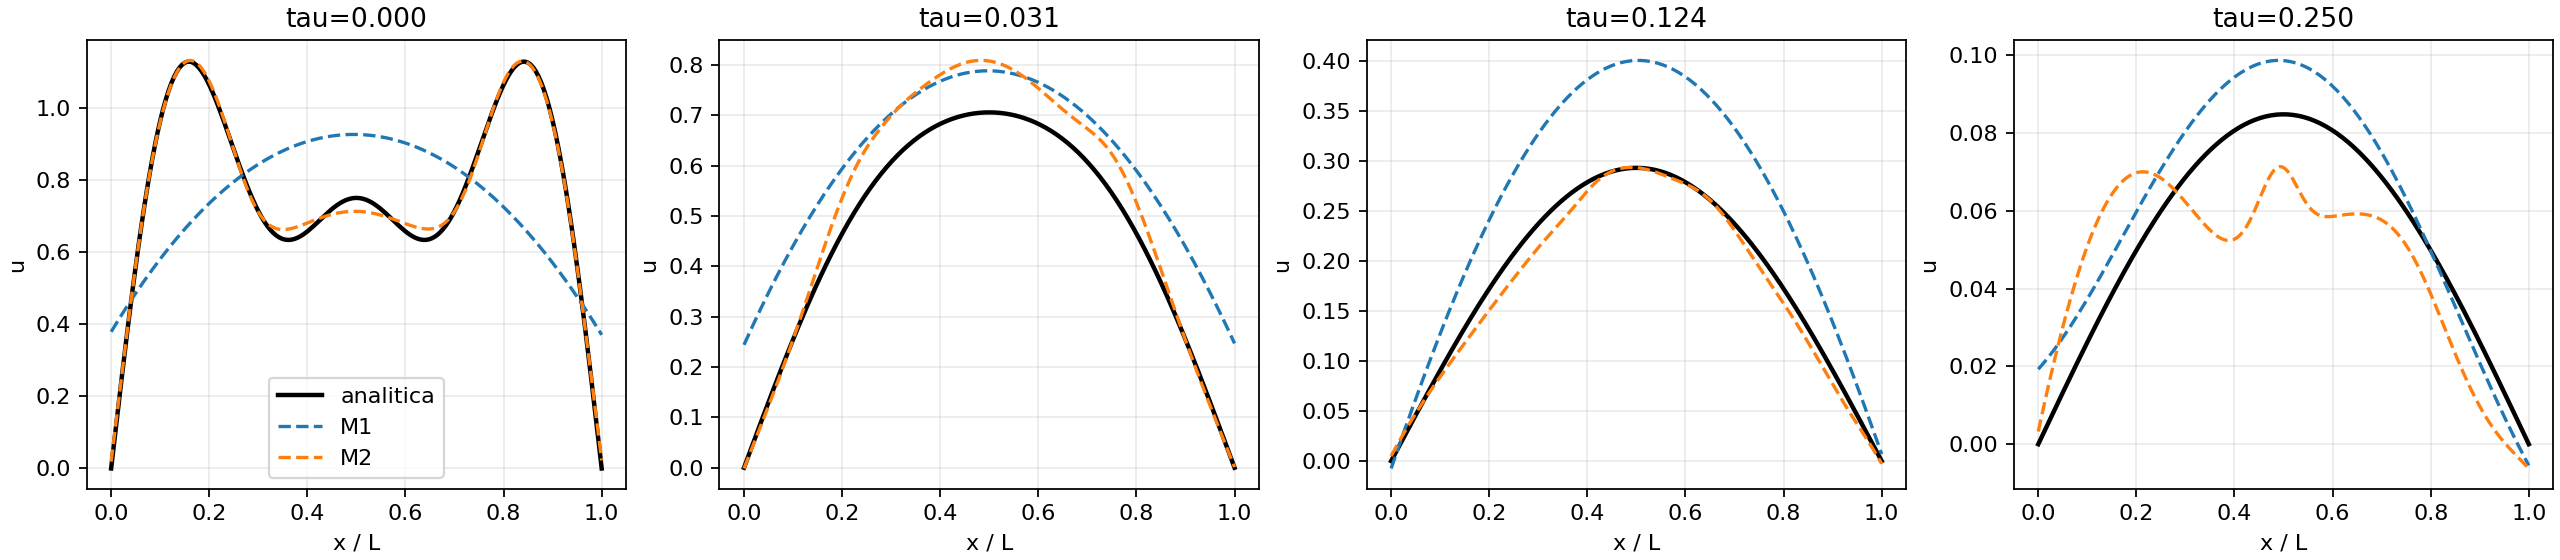
\includegraphics[width=\linewidth]{outputs/cortes_temporales.png}
\caption{Cortes espaciales en tiempos adimensionales fijos.}
\end{figure}

\section{Gradientes y sensibilidad}

Los histogramas de gradientes reproducen el analisis cualitativo del paper:
se inspeccionan los gradientes de $L_{\mathrm{res}}$, $L_{\mathrm{ic}}$ y
$L_{\mathrm{bc}}$ por capa para detectar desbalance entre terminos.

\begin{figure}[H]
\centering
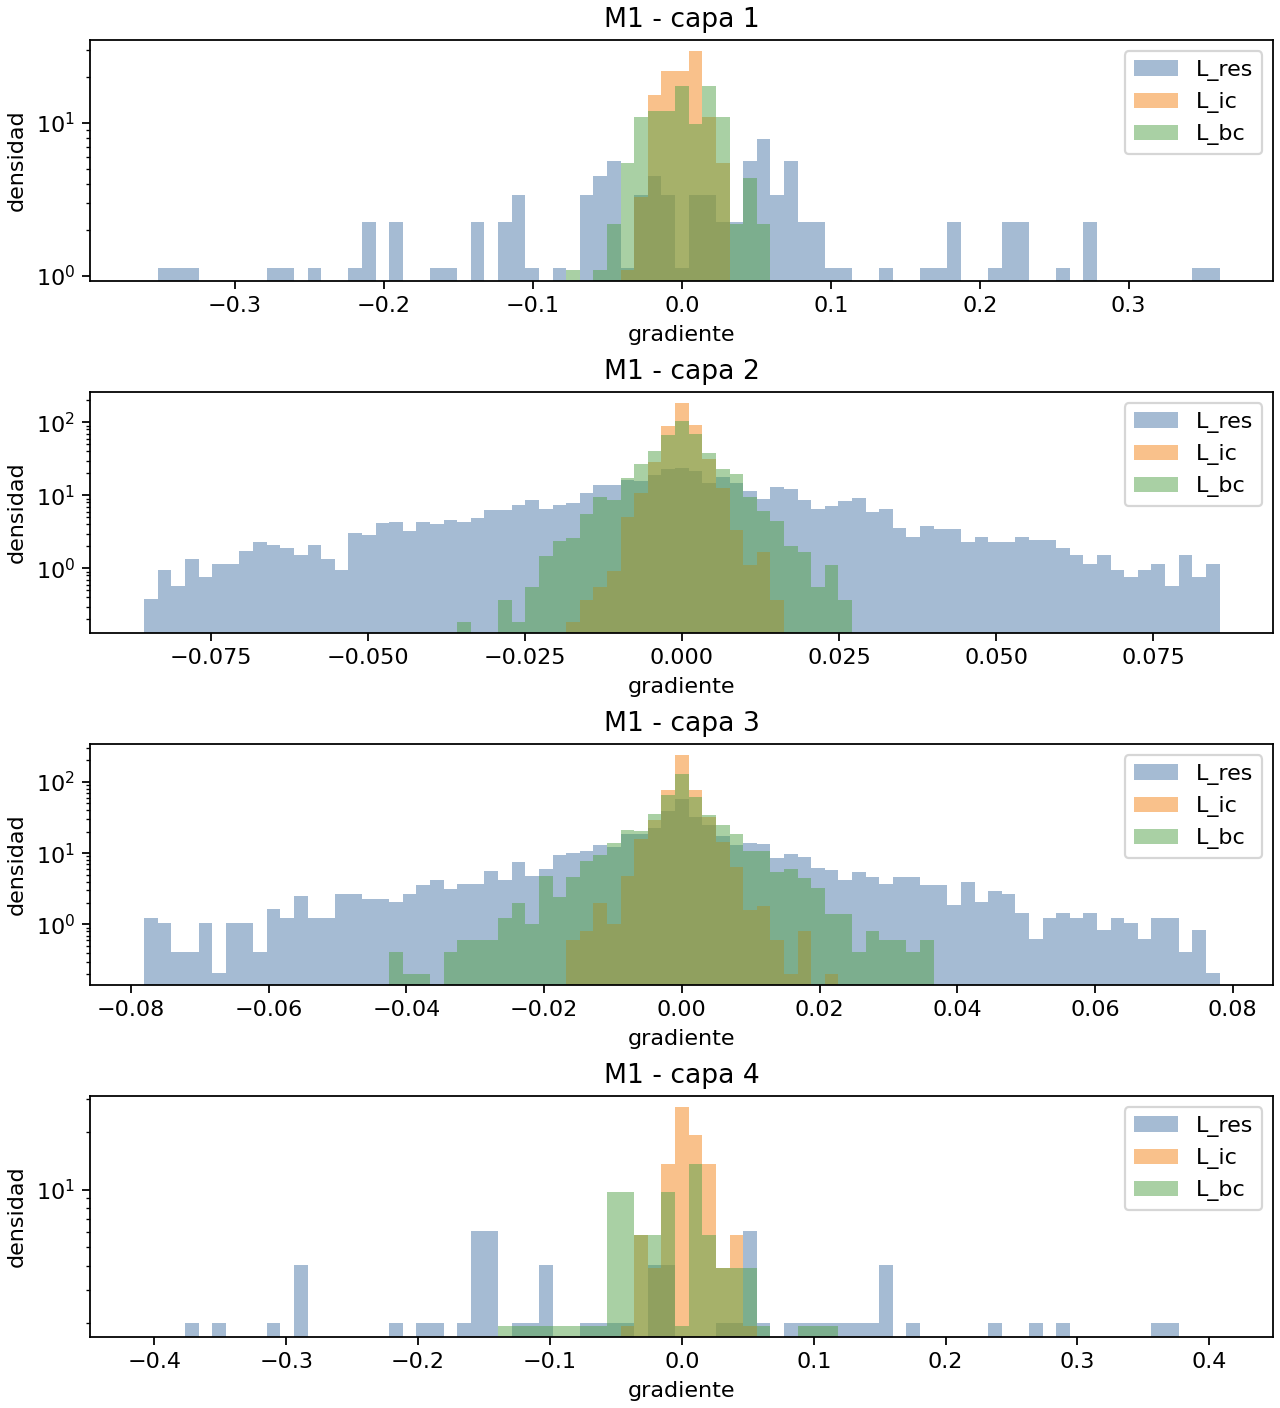
\includegraphics[width=0.82\linewidth]{outputs/M1_gradientes.png}
\caption{Histogramas de gradientes por capa para M1.}
\end{figure}

\begin{figure}[H]
\centering
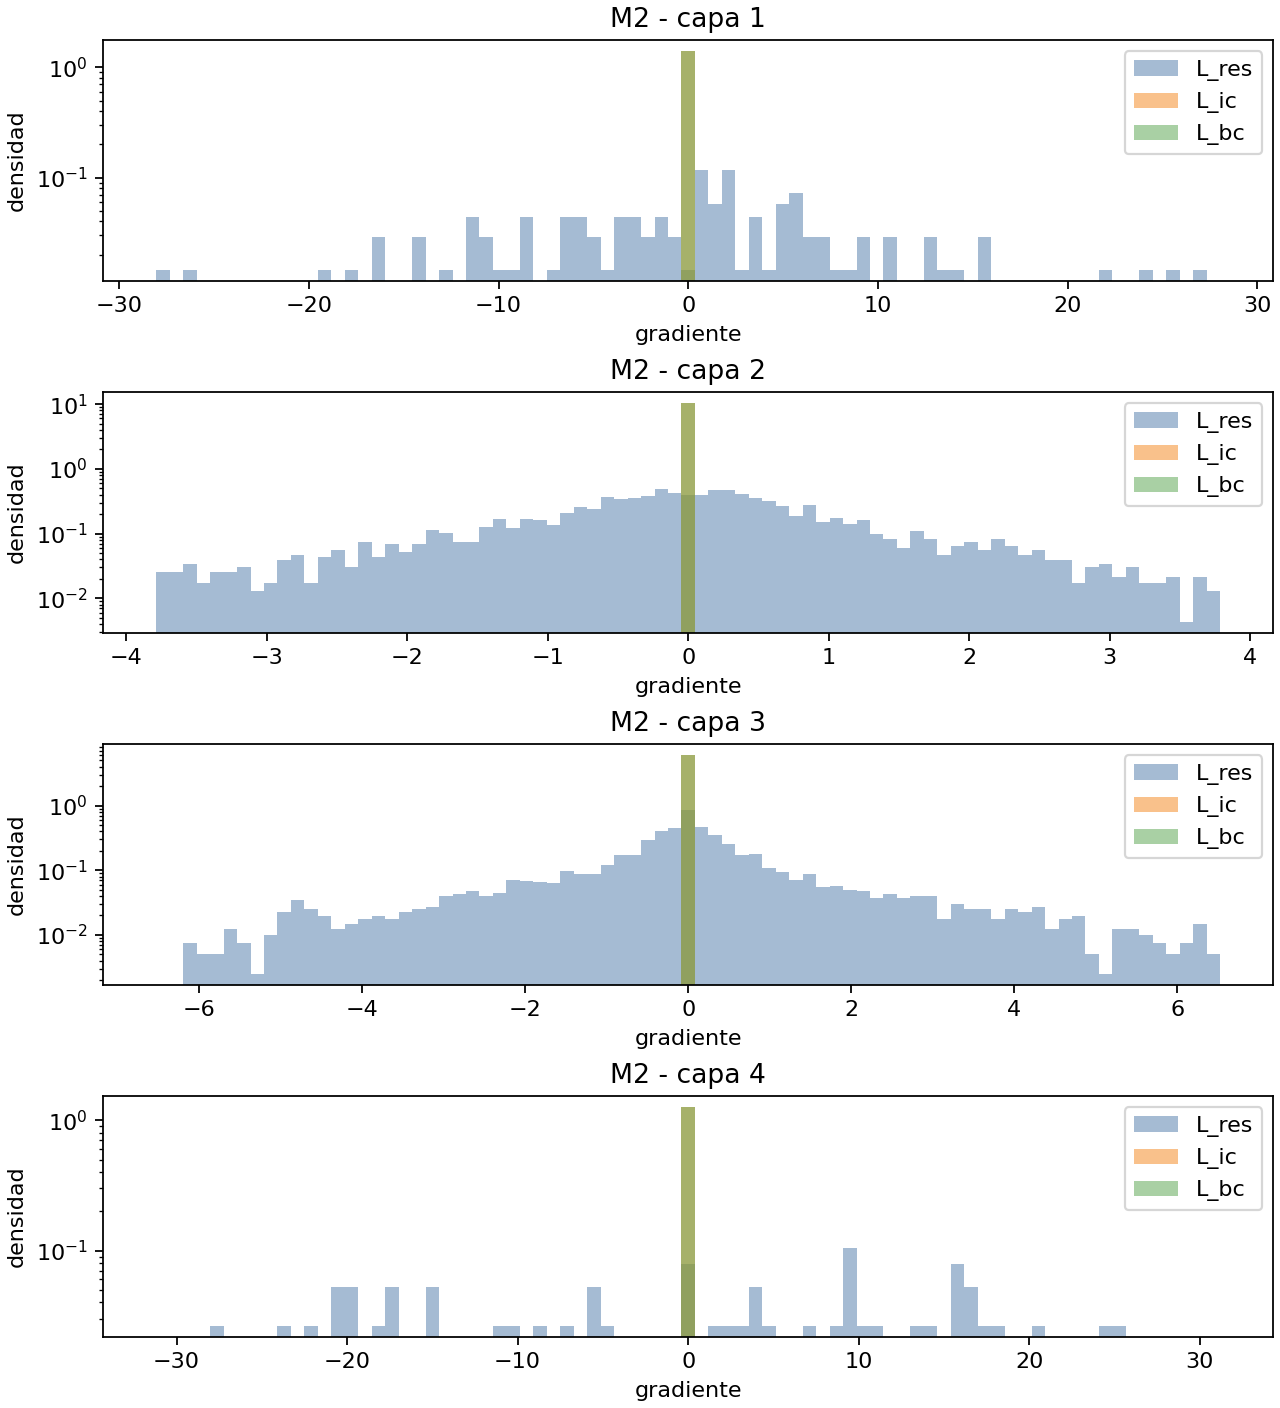
\includegraphics[width=0.82\linewidth]{outputs/M2_gradientes.png}
\caption{Histogramas de gradientes por capa para M2.}
\end{figure}

El mejor trial corto de la busqueda bayesiana tuvo
$\mathrm{width}=48$, $\mathrm{depth}=5$, $\eta=0.0010166$,
batch 384 y $\beta=0.76325$, con error corto 0.14138. Sin embargo, al validarlo
por 3000 iteraciones, los pesos adaptativos crecieron hasta orden $10^6$ y el
error final quedo en 0.18175 para M2. El regimen conservador con $\beta=0.9$
obtuvo 0.10291. Por eso la seleccion final no se baso solo en el mejor trial
corto, sino en validacion de estabilidad.

\begin{figure}[H]
\centering
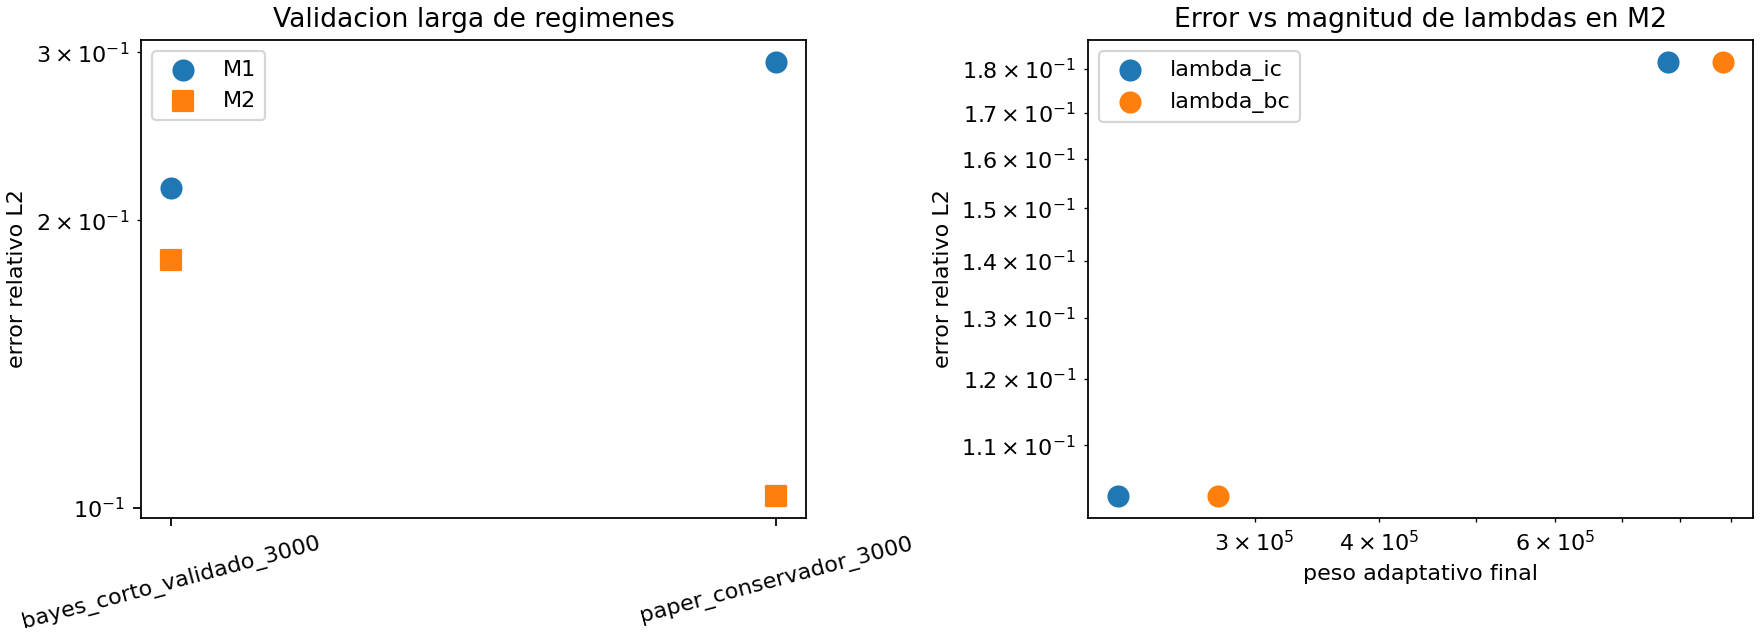
\includegraphics[width=\linewidth]{outputs/sensibilidad_regimenes.png}
\caption{Sensibilidad entre el mejor regimen bayesiano corto validado a 3000
iteraciones y el regimen conservador final.}
\end{figure}

\section{Busqueda bayesiana y optimizadores}

\begin{figure}[H]
\centering
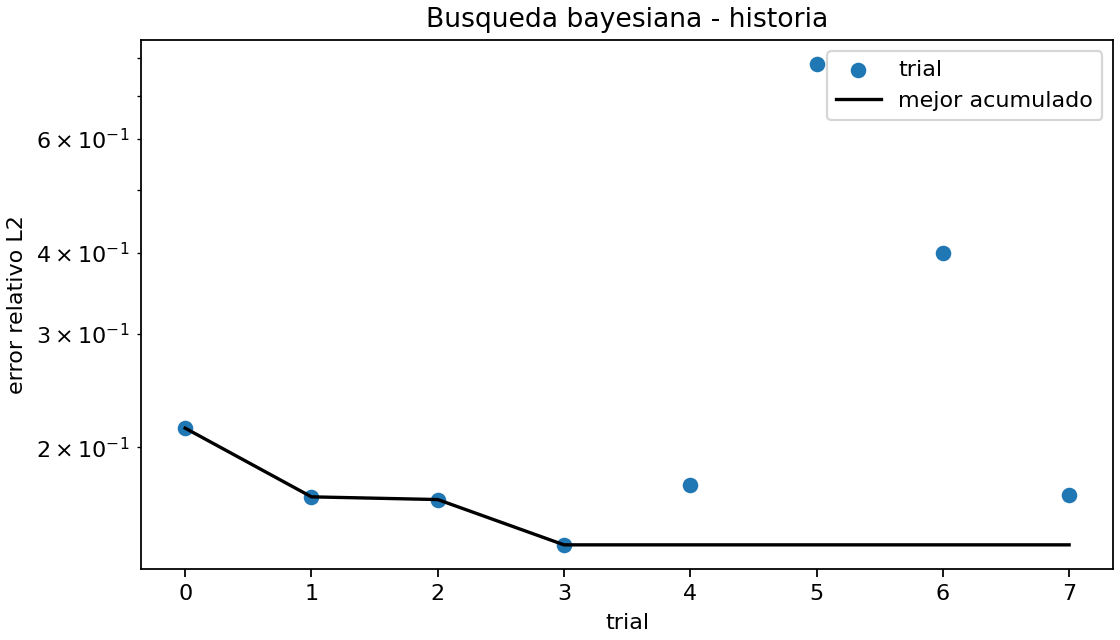
\includegraphics[width=0.82\linewidth]{outputs/bayes_historia.png}
\caption{Historia de trials y mejor error acumulado en la busqueda bayesiana.}
\end{figure}

\begin{figure}[H]
\centering
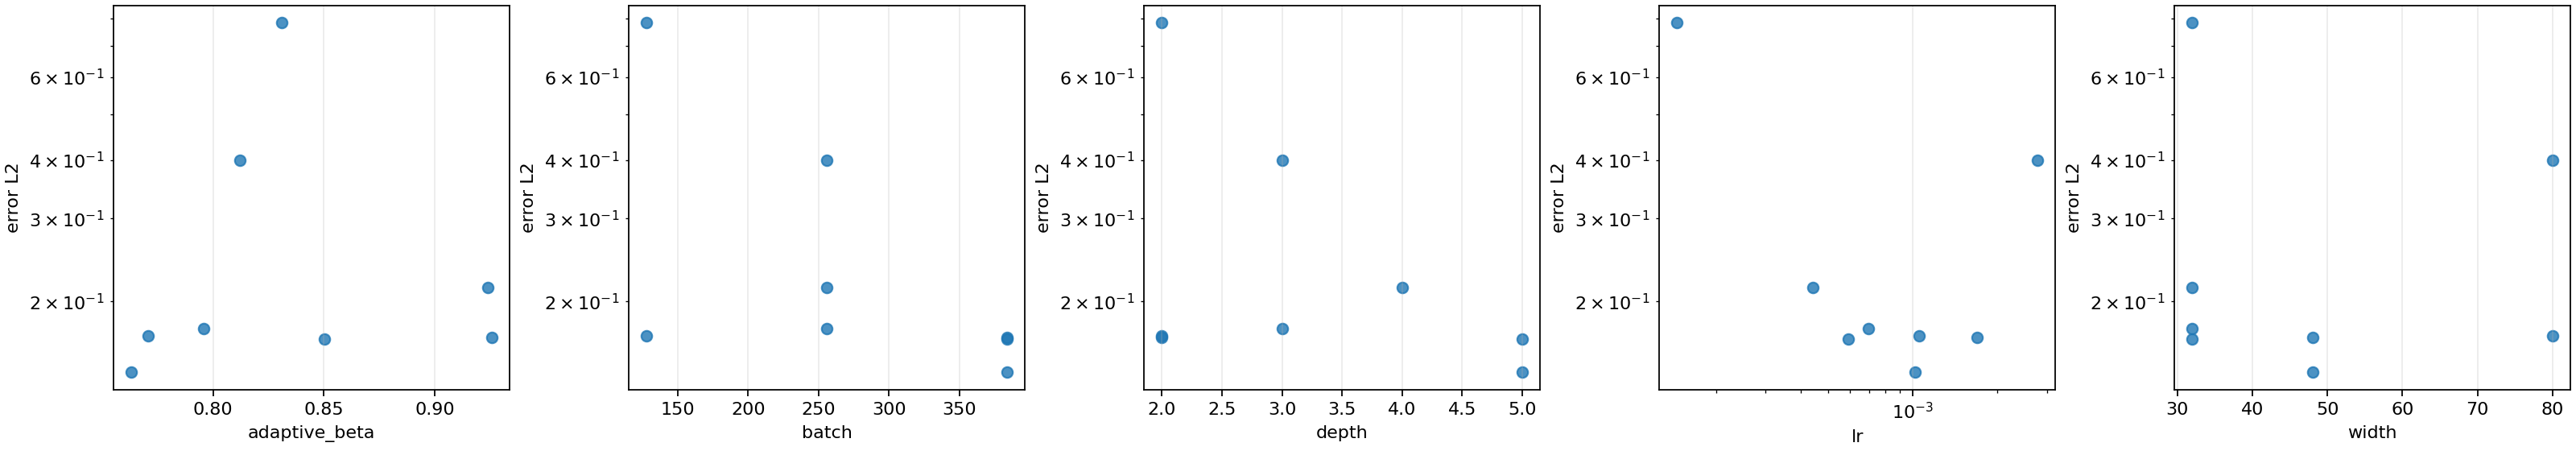
\includegraphics[width=\linewidth]{outputs/bayes_parametros.png}
\caption{Error contra parametros explorados por Optuna/TPE.}
\end{figure}

\begin{figure}[H]
\centering
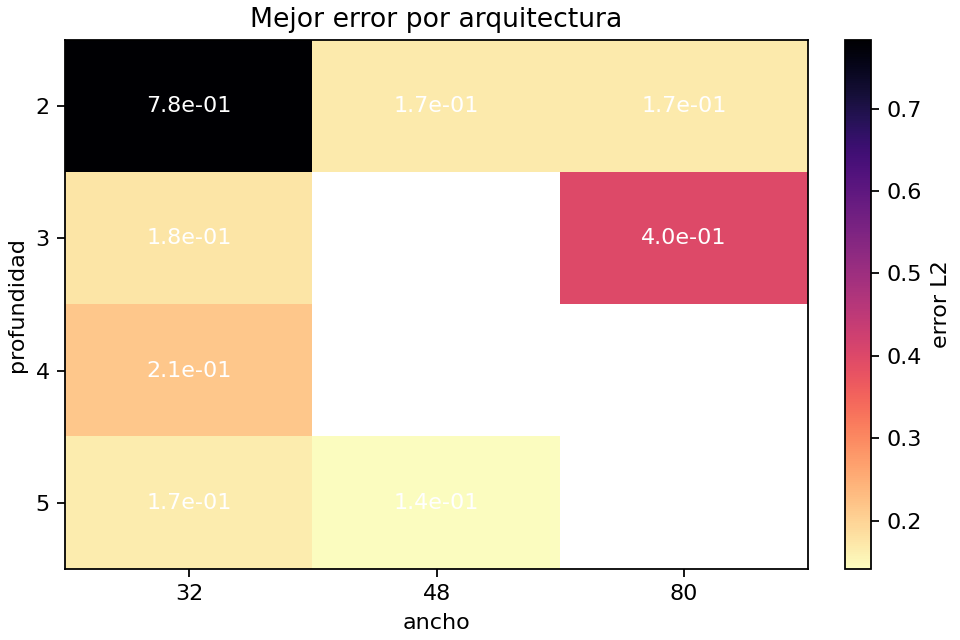
\includegraphics[width=0.72\linewidth]{outputs/bayes_heatmap_arquitectura.png}
\caption{Mejor error observado por ancho y profundidad.}
\end{figure}

La comparacion de optimizadores se hizo con presupuesto fijo y M2:
\begin{table}[H]
\centering
\begin{tabular}{lrr}
\toprule
Optimizador & error $L^2$ rel. & tiempo [s] \\
\midrule
Adam + LBFGS(10) & 0.166899 & 109.02 \\
Adam & 0.176340 & 122.15 \\
AdamW & 0.176340 & 71.27 \\
SGD & NaN & 116.69 \\
\bottomrule
\end{tabular}
\caption{Comparacion de optimizadores con 1000 iteraciones, batch 128 y
arquitectura $[2,32,32,32,1]$.}
\end{table}

\begin{figure}[H]
\centering

\includegraphics[width=0.72\linewidth]{outputs/comparacion_optimizadores.png}
\caption{Comparacion grafica de optimizadores. SGD divergio con el learning
rate comun usado en esta prueba.}
\end{figure}

\section{Reproducibilidad}

Los comandos principales fueron:
\begin{verbatim}
conda env create -f environment.yml
conda activate tp-optimizacion-ger

python experimento.py bayes --trials 8 --search-iters 800 --threads 16

python experimento.py todos \
  --iters 3000 --batch 256 --width 50 --depth 3 \
  --lr 0.001 --adaptive-beta 0.9 \
  --log-every 500 --nx 180 --nt 180 --threads 16

python experimento.py optimizadores \
  --iters 1000 --batch 128 --width 32 --depth 3 \
  --lr 0.001 --adaptive-beta 0.9 \
  --log-every 500 --nx 120 --nt 120 \
  --lbfgs-steps 10 --threads 16

python analisis_sensibilidad.py
tectonic reporte.tex
\end{verbatim}

\end{document}
